\documentclass{scrartcl}
\usepackage[utf8]{inputenc}
\usepackage{graphicx}
\usepackage{hyperref}

\def\theName{[protocol\_name]}

\hypersetup{
    colorlinks=true,
    linkcolor=blue,
    filecolor=magenta,
    urlcolor=cyan,
    pdftitle={\theName technical introduction},
    }

\title{\theName}
\subtitle{Hyper-parallelized on-chain order book for the Aptos blockchain}
\author{}
\date{\vspace{-55pt}} % Shift upwards since no author/date specified

\begin{document}

\maketitle

\begin{abstract}

\theName\ is a fully on-chain central limit order book, built on the Aptos blockchain.
Similar in form to \href{https://docs.google.com/document/d/1isGJES4jzQutI0GtQGuqtrBUqeHxl_xJNXdtOv4SdII}{Serum}, which is built on Solana, \theName\  introduces a key technical innovation that enables parallelism within a single trading pair:
the paraqueue.
This novel feature allows \theName\ to horizontally scale high-traffic markets, thus overcoming bottlenecks that have historically limited the throughput of automated market-makers and other blockchain-based order book exchanges.
As a trustless, permissionless, decentralized protocol, built on a high-performance web-scale blockchain, \theName\ is designed for a singular purpose:
to become the world’s premier price discovery engine.

\end{abstract}

\section{Write-locks and parallelism, order book tutorial style}

\subsection{Dual-market basic theory}

Consider two tokens, \texttt{ACE}, and \texttt{BED}, each trading against a tokenized version of the US dollar, in this case, \texttt{USDC}. The \href{https://guides.cryptowat.ch/trader-education/order-books-and-market-depth-charts-explained}{order books} for these two trading pairs are as follows:

\begin{center}
\resizebox{!}{3in}{%
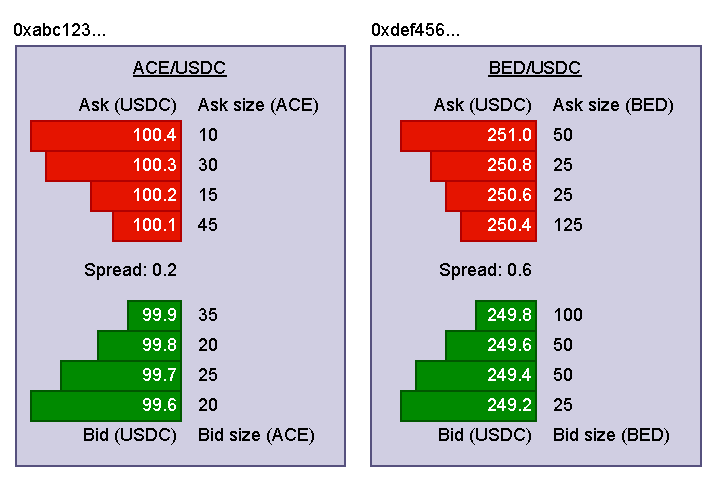
\includegraphics{two-books.pdf}%
}
\end{center}

Ignoring for the moment the exact data structures that comprise each order book, consider that the order book for the \texttt{ACE/USDC} pair is at address \texttt{0xabc123\ldots}, while the order book for the \texttt{BED/USDC} pair is at address \texttt{0x456def\ldots}, which means that \texttt{ACE/USDC} and \texttt{BED/USDC} trades can be executed in parallel.
For instance, if Art, with account address \texttt{0xdee789\ldots} wants to buy \texttt{ACE} using \texttt{USDC}, while Bud, with account address \texttt{0xfad321\ldots} wants to sell \texttt{BED} in exchange for \texttt{USDC}, both users' trades can clear in parallel.
For numerical simplicity, assume each \texttt{ACE} token trades for exactly 100 \texttt{USDC} (the nominal price corresponding to the above order book), and likewise, that each \texttt{BED} token trades for exactly 250 \texttt{USDC}:

\begin{center}
\resizebox{!}{4.5in}{%
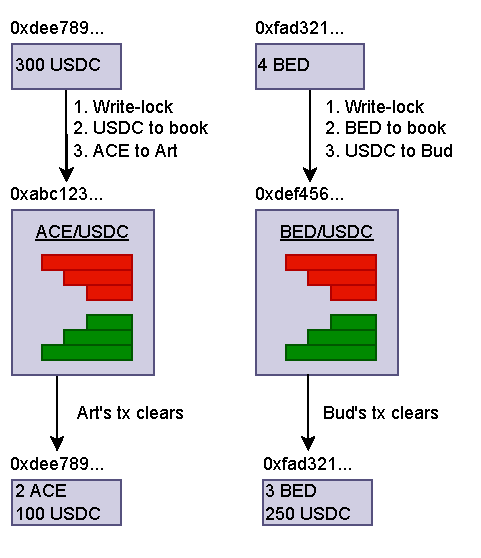
\includegraphics{parallel-pairs.pdf}%
}
\end{center}

On the left, Art starts off with 300 \texttt{USDC} and places an order to buy 2 \texttt{ACE} tokens.
The Aptos execution engine:

\begin{enumerate}
    \item Write-locks Art's address (\texttt{0xdee789\ldots}) and the address of the \texttt{ACE/USDC} order book (\texttt{0xabc123\ldots})
    \item Transfers 200 \texttt{USDC} from Art `to the order book' (explained in more detail below)
    \item Transfers 2 \texttt{ACE} from the order book to Art
\end{enumerate}

Art thus ends up with 2 \texttt{ACE} tokens and \texttt{USDC}.
Similarly, Bud starts off with 4 \texttt{BED} and places an order to sell 1 in exchange for \texttt{USDC}.
The Aptos execution engine:

\begin{enumerate}
    \item Write-locks Bud's address (\texttt{0xfad321\ldots}) and the address of the \texttt{BED/USDC} order book (\texttt{0xdef456\ldots})
    \item Transfers 1 \texttt{BED} from Bud `to the order book' (explained in more detail below)
    \item Transfers 250 \texttt{USDC} from the order book to Bud
\end{enumerate}

Bud thus ends up with 3 \texttt{BED} and 250 \texttt{USDC}.
Since these two operational sequences (Art's trade and Bud's trade) involve non-overlapping write-locks, they can be executed in parallel -- according to the overly-simplistic assumptions of this basic example.

\subsection{Settlement contention}

In reality, \texttt{USDC} does not transfer from Art `to the \texttt{ACE/USDC} orderbook', but rather, to the account that placed the limit order with the lowest asking price, e.g. 100.1 \texttt{USDC} per \texttt{ACE} token.
And if such a limit order happened to have been placed by Bud, who was trading on both markets, \texttt{ACE/USDC} and \texttt{BED/USDC}, then the parallelism as described above would not be possible.
Because if Bud has an outstanding limit order on the \texttt{ACE/USDC} market corresponding to the lowest ask, while Art tries to buy \texttt{ACE} and Bud simultaneously tries to sell \texttt{BED} on the \texttt{BED/USDC} market, then two execution sequences compete for a write-lock on Bud's address:

\begin{enumerate}
    \item Art's order to buy \texttt{ACE} would require write-locking Bud's account in order to pay out \texttt{USDC} to Bud against his outstanding limit order
    \item Bud's order to sell \texttt{BED} in exchange for \texttt{USDC} would require write-locking Bud's account in order to transfer \texttt{BED} out of his account
\end{enumerate}

Here, since Bud is trading on both markets, orders against each trading pair involve overlapping state -- Bud's account -- and parallelism breaks.
This problem is easily solved, though, by having each user register a separate account for each trading pair:

\begin{center}
\resizebox{!}{2.5in}{%
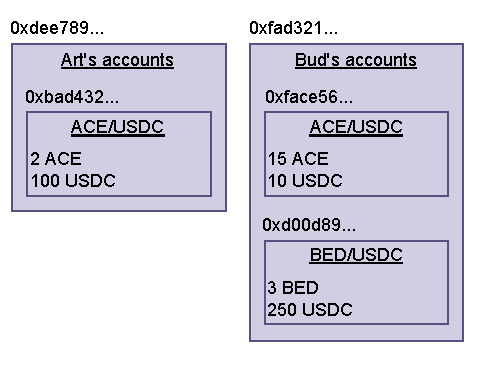
\includegraphics{user-accounts.pdf}%
}
\end{center}

Here, Bud retains his main account (address \texttt{0xfad321\ldots}), but registers an \texttt{ACE/USDC} trading account (address \texttt{0xface56\ldots}) and a separate \texttt{BED/USD} trading account (address \texttt{0xd00d89\ldots}).
Now, if he has an outstanding limit order on the \texttt{ACE/USDC} market, it can be filled at the same time that he places an order to sell \texttt{BED}, because the filling of his \texttt{ACE/USDC} limit order only needs to write-lock his \texttt{ACE/USDC} account, while his order to sell \texttt{BED} only needs to write-lock his \texttt{BED/USDC} account.
And although the above figure portrays Bud's accounts as nested, this is only for demonstrative purposes:
his main account (\texttt{0xfad321\ldots}) does not need to be write-locked when filling limit orders.
As for simple taker orders (buy/sell), it may be necessary to write-lock Bud's main account in addition to the corresponding market-specific account, depending on specific implementation details.
But this does not necessarily hinder system-wide parallelism, assuming orders are processed in a two-stage queue system that further isolates write-locks.

\subsection{Requests and events}

Since each order book contains limit orders from various users at various depths, it is impossible to determine, ahead of transaction processing time, which addresses will need to be write-locked in order to pay out against outstanding limit orders.
So in the above example, when Art placed an order to buy \texttt{ACE}, it actually would have been necessary to write-lock \emph{every single account} with an outstanding limit order (on the ask side).
This is because with a large enough order, Art could have emptied out 100\% of the depth in the order book, which would have entailed paying out to everyone who had placed a limit order (again, on the ask side).
Rather than write-locking every potential recipient of funds, a more efficient method of matching orders involves a two-stage queue system, where users submit `requests', and incentivized nodes trigger `events':

\begin{center}
\resizebox{!}{3.5in}{%
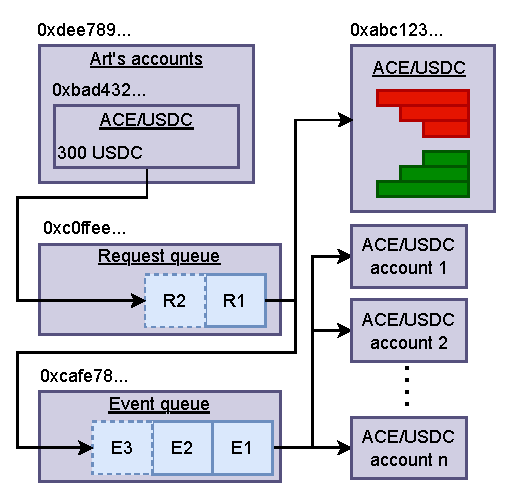
\includegraphics{two-queues.pdf}%
}
\end{center}

Here, when Art decides to buy \texttt{ACE} using \texttt{USDC}, he submits an order request to a first-in-first-out (FIFO) queue (address \texttt{0xc0ffee\ldots}).
The protocol smart contract performs validity checks to ensure that his order request is properly formatted, and his request is inserted at the back of the queue, as request object \texttt{R2}.
Assuming Art's order request passes validity checks, his funds are deposited into the request queue, after which they will be processed in deterministic fashion according to protocol logic, whereas if Art's order request is improperly formatted, the transaction errors out and his funds are returned.
At most, this operation requires a write-lock on the following addresses:

\begin{enumerate}
    \item Art's main account (\texttt{0xdee789\ldots})
    \item Art's \texttt{ACE/USDC} account (\texttt{0xbad432\ldots})
    \item The request queue (\texttt{0xc0ffee\ldots})
\end{enumerate}

Eventually Art's request will move to the front of the queue, which is monitored by a network of incentivized nodes.
In return for protocol fees, these nodes issue transactions that trigger the protocol's matching engine, which is contained completely within smart contract logic, such that nodes never have control over users' funds -- again, once funds have made their way into the request queue, they proceed according to deterministic smart contract logic.
Limit (maker) orders are added to the book, (taker) buys and sells are matched against limit orders, order cancellations are taken off the book, and other order types (immediate-or-cancel, post-only, etc.) are processed accordingly, leading to the generation of `events'.
An event describes the amount of funds to be administered to any and all accounts affected by a request, and allows event-processing logic to pre-construct transactions that only write-lock the minimum number of addresses.

When the request at the front of the request queue, \texttt{R1} is processed, the following addresses are write-locked:

\begin{enumerate}
    \item The request queue (\texttt{0xc0ffee\ldots})
    \item The order book (\texttt{0xabc123\ldots})
    \item The event queue (\texttt{0xcafe78\ldots})
    \item The account of the triggering node
\end{enumerate}

Funds are transferred to the event queue, either from the request queue, the order book, or both, and a new entry, \texttt{E3}, is inserted at the back of the event queue.

Similarly, nodes send transactions that trigger the processing of events, like \texttt{E1} as shown above, in which they pre-declare the addresses that will need to be write-locked for the deterministic smart contract logic to disperse funds.
Again, nodes are only sending a transaction that triggers logic contained purely within the protocol smart contract, except in this case they are additionally pre-declaring the addresses that will need to be write-locked:
\texttt{ACE/USDC} account 1, \texttt{ACE/USDC} account 2, \ldots, up to \texttt{ACE/USDC} account n in the above example.
Through this two-queue system, an arbitrary number of trading pairs can be processed in parallel, with each market write-locking the minimum number of addresses.

However, within a single trading pair, order requests are still serialized, because all users write to the same request queue for the given market.
Especially for high-traffic trading pairs, this design deficiency leads to performance bottlenecks at the request queue, inhibiting market throughput and price discovery.

Through a novel form of parallelism, \theName\ solves this dilemma.

\subsection{Paraqueues}

\begin{center}
\resizebox{!}{3.5in}{%
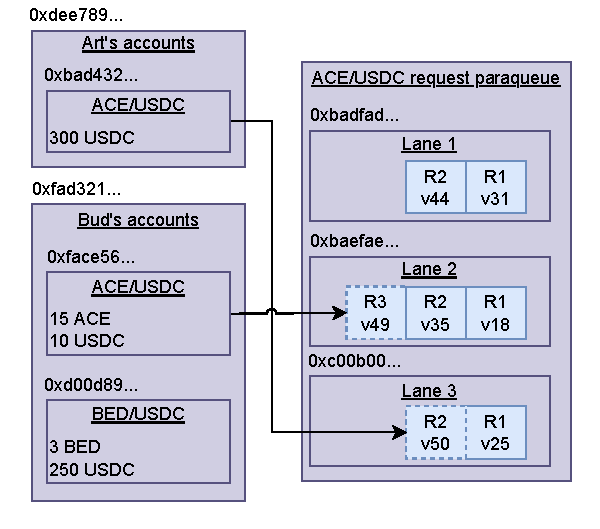
\includegraphics{paraqueue.pdf}%
}
\end{center}

In this arrangement, \texttt{ACE/USDC} order requests are sent to a `paraqueue' with 3 `lanes', where request objects in each lane are encoded with the \href{https://aptos.dev/basics/basics-txns-states/#versioned-database}{Aptos database version number} of the state against which the corresponding request transaction was executed:
in the above example, for instance, request object \texttt{R1} in lane 1 corresponds to version number 31.
For each request transaction, a hash on the transaction payload -- excluding the destination address -- henceforth referred to as a quasi-hash, is used to determine which paraqueue it should be sent to, with quasi-hashes bucketed according to the number of lanes in the paraqueue:
for the above diagram, in a simplified example, if a hashing function outputs an integer between 1 and 120 (inclusive), then request transactions with a quasi-hash between 1 and 40 should be addressed to lane 1, request transactions with a quasi-hash between 41-80 should be addressed to lane 2, and request transactions with a quasi-hash between 81-120 should be sent to lane 3.
Validity checks on order requests reject transactions sent to the wrong paraqueue lane, to the effect that in aggregate, request objects will be near-uniformly distributed across all lanes (since hash functions are practically random for this purpose), thus increasing throughput by a factor of $ n $, where $ n $ is the number of lanes.

In the above example, Art sends a request transaction to lane 3 (\texttt{0xc00b00\ldots}) while Bud simultaneously sends a request transaction to lane 2 (\texttt{0xbaefae\ldots}), with each such transaction write-locking non-overlapping state.
Hence the two transactions can be cleared in parallel, with their chronology preserved via the \href{https://aptos.dev/basics/basics-txns-states/#versioned-database}{Aptos database version number} encoded in each request object.
Thus, when nodes pop requests off the front of the paraqueue, they can re-order transactions from all of the lanes within, according to version numbers, preserving the chronology of requests.
By batching up requests according to this chronology, nodes can process requests into events that condense the execution results of multiple orders, thus preserving the higher throughput enabled by request paraqueues.
Additionally, nodes can dynamically expand or contract the number of lanes within a given paraqueue (again, without invalidating orders or seizing funds) based on traffic, allowing for maximum horizontal scaling across high-traffic markets.

\end{document}
